\section{Introducción}
\bigskip

El presente informe detalla el diseño e implementación de un amplificador de audio clase G. En la realización de este proyecto han sido volcados los conocimientos de la materia Circuitos Electrónicos II. En la Figura~\ref{esquema_bloques}, se muestra el diagrama en bloques de las partes fundamentaes del proyecto.
	
	\begin{figure}[H]
	\centering
	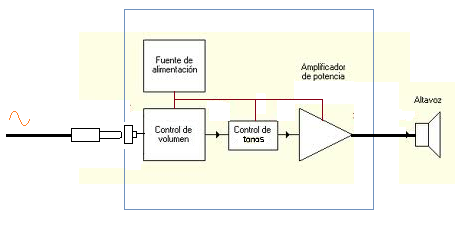
\includegraphics[scale=0.65]{img/esquema_bloques.png}
	\caption{Esquema en bloques.}
	\label{esquema_bloques} 
	\end{figure}
	
	
Un preamplificador es un circuito que permite adaptar las diferentes señales de entrada para luego poder ingresarlas a una etapa de potencia. Este circuito puede servir para adaptar señales de diferentes fuentes, por ejemplo: micrófonos, reproductores de mp3, salidas de placas de sonido de  pc, etc. Como todos estos dispositivos no tienen el mismo nivel de salida, el preamplificador es quien se encarga de llevar a todas estas señales a una tensión de estipulada que luego entra a la etapa de potencia anteriormente nombrada. Los preamplificadores suelen ser de baja potencia y de realizarse de forma adecuada no deben distorsionar en gran medida la señal.

Alguno de los controles que pueden tener los preamplificadores son:
	
\begin{itemize}
	\item Control de volumen
	\item Control de tono
	\item Control de balance
	\item Selector de canal de entrada 
	\item Amplificación
	\end{itemize}	
	
Un amplificador debe satisfacer ciertos requerimientos especiales. Uno de los más importantes es el de entregar una señal con una cantidad específica de potencia a una carga con niveles aceptablemente bajos de distorsión. Otro objetivo común en el diseño es minimizar la impedancia de salida, de tal forma que la ganancia de voltaje quede relativamente poco afectada por el valor de la impedancia de carga. Una etapa de salida bien diseñada debe cumplir con estas características de funcionamiento, consumiendo poca potencia en estado de reposo, sin que esto represente una limitación importante en la respuesta en frecuencia del amplificador. 
 

Los amplificadores de potencia  se clasifican generalmente en seis tipos: A, B, AB , C y G para diseños analógicos y clases D y E para los diseños de conmutación. 

\subsubsection*{Amplificadores clase A.}
\medskip 

En esta clase de amplificadores se usa un solo transistor. El emisor seguidor es la etapa de salida clase A mas utilizada. La corriente de salida circula durante todo el ciclo de la señal de entrada, ya que el transistor esta polarizado con una corriente continua. Esta es una de las grandes desventajas de este tipo de amplificador ya que consume potencia en ausencia de señal y por lo tanto es lógico esperar un rendimiento pobre que en general no supera el 25\%. Como ventaja la distorsión introducida suele ser baja. En la Figura~\ref{ampliA} se muestra un ejemplo de este tipo de amplificador.
 
\begin{figure}[H]
\centering
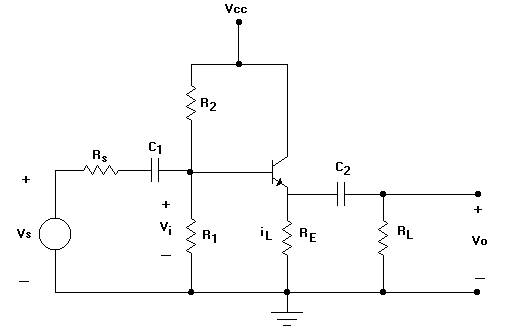
\includegraphics[scale=0.6]{img/ampliA.png}
\caption{Ejemplo, amplificador clase A}
\label{ampliA} 
\end{figure}

\subsubsection*{Amplificador clase B}
\medskip 

Esta clase de amplificadores se compone de un par de transistores (uno pnp y otro npn) conectados de forma tal que no se encuentren ambos en la zona de modo activo directo en el mismo instante de tiempo. Es decir, si suponemos tener una entrada senoidal, durante un semiciclo uno de los transistores se encuentra en la región activa, conduciendo corriente, mientras que el otro se encuentra en corte y durante el otro semiciclo viceversa.
 Una ventaja de esta amplificador sobre la clase A, es que los transistores no disipan potencia en ausencia de señal, lo cual mejora la vida util de los transistores y el rendimiento notablemente, alcanzando un máximo del 78\%.
 La desventaja en este tipo de amplificadores es la llamada “distorsión por cruce”. Es fácil detectar su procedencia al analizar la Figura~\ref{ampliB}.

\begin{figure}[H]
\centering
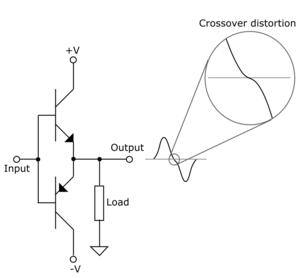
\includegraphics[scale=0.8]{img/ampliB.png}
\caption{Ejemplo, salida clase B.}
\label{ampliB} 
\end{figure}




El desarrollo del trabajo fue encarado como un caso real de la vida profesional, en el cual se nos han dado las especificaciones y basamos en ellas nuestro diseño, tratando de ser lo mas eficientes al menor costo posible y con los productos que se pudieron encontrar en el mercado.
	
Durante el desarrollo del trabajo hemos ido encontrando inconvenientes, ya sea errores humanos o diferencias entre las simulaciones y la implementación material. Se detallaron dichos problemas ya que consideramos que contribuyen al proceso de aprendizaje del diseño real.